\documentclass[11pt,a4paper]{article}

% --- Packages ---
\usepackage[utf8]{inputenc}
\usepackage[T1]{fontenc}
\usepackage{lmodern}
\usepackage[margin=1in,headheight=14pt]{geometry}
\usepackage{amsmath,amssymb}
\usepackage{booktabs}
\usepackage{tabularx}
\usepackage{longtable}
\usepackage{array}
\usepackage{xcolor}
\usepackage{graphicx}
\usepackage{fancyhdr}
\usepackage{titlesec}
\usepackage{enumitem}
\usepackage{tcolorbox}
\usepackage{tikz}
\usetikzlibrary{shapes.geometric,arrows.meta,positioning,calc,shadows.blur}
\usepackage{hyperref}
\usepackage{microtype}
\usepackage{cite}
\usepackage{float}

% --- Color Palette (Modern Academic Navy & Slate) ---
\definecolor{primary}{RGB}{20, 50, 95}       % Deep Oxford Navy
\definecolor{secondary}{RGB}{41, 128, 185}   % Academic Blue
\definecolor{accent}{RGB}{230, 126, 34}      % Amber Accent
\definecolor{darkslate}{RGB}{44, 62, 80}     % Dark Slate
\definecolor{lightbg}{RGB}{247, 249, 252}    % Soft Gray-Blue
\definecolor{bordercolor}{RGB}{210, 220, 230}% Border Gray
\definecolor{badgegreen}{RGB}{39, 174, 96}   % Verified Green
\definecolor{badgered}{RGB}{192, 57, 43}     % Alert Red

% --- Hyperref Setup ---
\hypersetup{
    colorlinks=true,
    linkcolor=primary,
    citecolor=secondary,
    pdfauthor={Abu Zafor (232-35-331), Anamul Haque (232-35-285)},
    pdftitle={UniExpert: AI-Powered Expert Discovery and Academic Collaboration Platform},
    pdfsubject={SE 331 Software Engineering Design Capstone Project Proposal},
    pdfkeywords={Expert Discovery, AI Recommendation, Semantic Search, Capstone Proposal, Academic Collaboration}
}

% --- Header and Footer Styling ---
\pagestyle{fancy}
\fancyhf{}
\fancyhead[L]{\small\textbf{\textcolor{primary}{UniExpert}} \textcolor{gray}{\,$|$\,} \textcolor{darkslate}{SE 331 Capstone Proposal}}
\fancyhead[R]{\small\textcolor{darkslate}{\nouppercase{\leftmark}}}
\fancyfoot[L]{\small\textcolor{gray}{Confidential -- Academic Capstone Evaluation}}
\fancyfoot[R]{\small\thepage}
\renewcommand{\headrulewidth}{0.6pt}
\renewcommand{\footrulewidth}{0.4pt}

% --- Section Title Formatting ---
\titleformat{\section}
  {\Large\bfseries\color{primary}}{\thesection}{1em}{}[\titlerule]
\titleformat{\subsection}
  {\large\bfseries\color{darkslate}}{\thesubsection}{1em}{}
\titleformat{\subsubsection}
  {\normalsize\bfseries\color{secondary}}{\thesubsubsection}{1em}{}

% --- TColorBox Styling ---
\tcbuselibrary{skins,breakable}
\newtcolorbox{calloutbox}[2][]{
    colback=lightbg,
    colframe=primary,
    coltitle=white,
    title=\textbf{#2},
    fonttitle=\bfseries,
    sharp corners,
    boxrule=1pt,
    arc=3pt,
    breakable,
    #1
}
\newtcolorbox{examplebox}[1][]{
    colback=white,
    colframe=secondary!80!black,
    fonttitle=\bfseries,
    coltitle=white,
    title=\textbf{Case Example},
    sharp corners,
    boxrule=0.8pt,
    arc=2pt,
    breakable,
    #1
}

% --- Custom Environments & Commands ---
\newcommand{\reqtag}[1]{\textsf{\textbf{\textcolor{primary}{[#1]}}}}
\newcommand{\statustag}[2]{\colorbox{#1!15}{\textcolor{#1}{\textbf{\small #2}}}}

\setlist[itemize]{noitemsep, topsep=3pt, parsep=2pt}
\setlist[enumerate]{noitemsep, topsep=3pt, parsep=2pt}

% ==============================================================================
% DOCUMENT BEGINS
% ==============================================================================
\begin{document}

% ------------------------------------------------------------------------------
% TITLE PAGE
% ------------------------------------------------------------------------------
\begin{titlepage}
    \centering
    \vspace*{1.2cm}
    
    {\large\scshape Department of Software Engineering}\\[0.2cm]
    {\normalsize Faculty of Science \& Information Technology}\\[2.2cm]
    
    {\Huge\bfseries\color{primary} UniExpert}\\[0.5cm]
    {\LARGE\bfseries\color{darkslate} AI-Powered Expert Discovery and Academic Collaboration Platform}\\[0.8cm]
    {\large\color{secondary} Capstone Project Proposal}\\[0.4cm]
    \rule{3.2in}{0.5pt}\\[0.6cm]
    
    {\normalsize\textbf{Course:} SE 331 --- Software Engineering Design Capstone Project}\\[0.25cm]
    {\normalsize\textbf{Semester:} Fall 2026 \quad $\cdot$ \quad \textbf{Duration:} October -- December 2026}\\[3.2cm]
    
    \begin{minipage}[t]{0.48\textwidth}
        \begin{flushleft}
            {\small\scshape Prepared By (Student Team)}\\[0.35cm]
            \textbf{Abu Zafor}\\
            {\small Student ID: 232-35-331}\\[0.25cm]
            \textbf{Anamul Haque}\\
            {\small Student ID: 232-35-285}
        \end{flushleft}
    \end{minipage}
    \hfill
    \begin{minipage}[t]{0.45\textwidth}
        \begin{flushright}
            {\small\scshape Supervised By}\\[0.35cm]
            \textbf{Mr. Md. Shohel Arman}\\[0.12cm]
            {\small Assistant Professor}\\
            {\small Department of Software Engineering}
        \end{flushright}
    \end{minipage}
    
    \vfill
    
    {\small\textbf{Date of Submission:} October 12, 2026}
    \vspace*{1.0cm}
\end{titlepage}

% ------------------------------------------------------------------------------
% EXECUTIVE SUMMARY / ABSTRACT
% ------------------------------------------------------------------------------
\thispagestyle{plain}
\section*{Executive Summary}
\addcontentsline{toc}{section}{Executive Summary}

Undergraduate and graduate students undertaking capstone projects, theses, and innovative research consistently face a systemic operational bottleneck: identifying and initiating collaboration with domain-specific experts, interdisciplinary researchers, and experienced industry mentors. Traditional institutional directories, keyword-based search tools, and siloed academic websites fail to bridge this divide. Students often lack formal knowledge of academic taxonomic titles (e.g., knowing whether a problem requires a computer vision specialist, a biostatistician, or a bioinformatics researcher) and have limited professional networks, while experts are inundated with vague, poorly matched solicitations.

To address this challenge, this capstone proposal introduces \textbf{UniExpert}, an intelligent, AI-powered expert discovery and academic collaboration platform. UniExpert combines natural language requirement parsing, dense semantic embeddings, multi-criteria hybrid ranking, and an automated research team builder to connect student research problems with verified academic and industrial specialists across all major domains. Rather than searching solely by fixed keywords, students input unstructured, natural language problem descriptions. UniExpert extracts primary and secondary domains, technical skill prerequisites, and research scopes, subsequently mapping these requirements to a curated and verified expert corpus. Recommendations are ranked using a hybrid scoring model integrating domain relevance, skill overlap, research interest similarity, verified credentials, availability, and collaboration preferences, complete with explainable natural language rationale.

The engineering and research scope of this Fall 2026 capstone project (October -- December 2026, 12 weeks) encompasses: (1) design and implementation of a scalable full-stack web application; (2) construction of a hybrid recommendation pipeline; (3) an empirical comparative study evaluating the hybrid engine against classical BM25 keyword matching and dense vector retrieval; and (4) structured verification and safety workflows tailored to academic integrity.

\vspace{0.8cm}
\begin{calloutbox}{Project Quick Reference Card}
\begin{tabularx}{\textwidth}{@{}lX@{}}
\textbf{Project Name:} & \textbf{UniExpert} (AI-Powered Academic Collaboration Platform) \\
\textbf{Target Users:} & University Students, Professors, Researchers, Industry Mentors, Admins \\
\textbf{Core Innovation:} & Problem-driven Natural Language Querying, Hybrid Multi-Criteria Matching, Multi-Tier Evidence Verification, and Explainable Team Assembly \\
\textbf{Primary Research Question:} & \textit{Does hybrid AI-based expert matching provide statistically significant higher relevance and user conversion than keyword retrieval and semantic similarity alone?} \\
\textbf{Evaluation Metrics:} & Precision@5, Recall@5, NDCG@5, Skill Extraction F1, Latency, Conversion Rate \\
\textbf{Primary Deliverables:} & Full-stack platform, reproducible AI pipeline, benchmark dataset, research paper.
\end{tabularx}
\end{calloutbox}

\newpage
% ------------------------------------------------------------------------------
% TABLE OF CONTENTS & LISTS
% ------------------------------------------------------------------------------
\tableofcontents
\vspace{0.5cm}
\listoffigures
\vspace{0.5cm}
\listoftables
\newpage

% ------------------------------------------------------------------------------
% SECTION 1: PROJECT OVERVIEW & PROBLEM STATEMENT
% ------------------------------------------------------------------------------
\section{Project Overview and Problem Statement}

\subsection{Background and Academic Context}
In modern higher education, academic projects---such as final-year capstones, honours theses, and independent research initiatives---are increasingly interdisciplinary. A biomedical device requires expertise in both embedded systems and physiological sensors; an agricultural prediction system combines machine learning with poultry pathology; and a financial analysis tool requires both software architecture and quantitative econometric modeling. 

Despite this interdisciplinary reality, university mentoring structures remain overwhelmingly siloed within distinct academic faculties. Students are typically restricted to consulting the immediate faculty members of their home departments. When an academic project ventures beyond departmental boundaries, students face severe friction in discovering, vetting, and contacting appropriate experts.

\subsection{The Core Problem Statement}
The core problem addressed by \textbf{UniExpert} is formulated as follows:
\begin{quote}
\textit{University students frequently struggle to identify, evaluate, and establish collaboration with domain-specific experts, researchers, and professional mentors whose specialized knowledge is essential for the completion and academic rigor of their research, thesis, and capstone projects.}
\end{quote}

This systemic failure stems from four distinct structural deficiencies:
\begin{enumerate}[label=\textbf{(\arabic*)}]
    \item \textbf{The Vocabulary Mismatch Problem:} Students understand their project goals in plain language but rarely know the precise academic nomenclature, taxonomies, or specialized credentials required (e.g., searching for ``poultry disease AI'' instead of ``computational epidemiology and computer vision for livestock welfare''). Keyword-based systems fail under this vocabulary divergence.
    \item \textbf{Fragmentation and Cold Outreach Overhead:} Expert information is scattered across disparate sources: institutional staff directories, personal websites, Google Scholar profiles, LinkedIn, and GitHub repositories. Students resort to speculative cold emails, which frequently lack context, leading to high rejection and ignore rates.
    \item \textbf{Absence of Verification and Credential Distrust:} Self-reported claims on generic professional networks cannot differentiate between actual peer-reviewed research publications, accredited institutional degrees, and superficial familiarity, exposing students to unverified advice.
    \item \textbf{Multidisciplinary Team Bottlenecks:} Multi-faceted projects require cohesive teams of complementary specialists rather than a single advisor. Students lack automated tools to detect team skill gaps and assemble multidisciplinary advisory panels.
\end{enumerate}

\subsection{The Proposed Solution: UniExpert}
\textbf{UniExpert} resolves these challenges by introducing an end-to-end, AI-powered expert discovery and academic collaboration platform. The system operates on a \textit{problem-first paradigm}: students articulate their project goals using unstructured natural language, and the underlying AI architecture parses, decomposes, and contextualizes these requirements. It matches the project against a database of verified experts from academia, research institutions, and industry, scoring candidates based on multi-dimensional compatibility and generating transparent, explainable recommendations.

\subsection{Scope Boundaries and Non-Goals}
A critical engineering principle for this capstone is strict scope discipline. UniExpert is deliberately designed with specific boundaries:
\begin{itemize}
    \item \textbf{In-Scope:} Problem parsing, semantic search, hybrid multi-criteria ranking, explainable recommendation justifications, multi-tier credential verification, project postings, structured collaboration requests, and workspace communication channels.
    \item \textbf{Explicit Non-Goals (Out of Scope for MVP):} UniExpert will \textbf{not} attempt to be a general open social network, a freelance gig-work financial marketplace, a real-time multi-party video conferencing engine (Zoom clone), or a full-fledged laboratory management suite. Its sole focus remains on \textit{accurate, trust-verified expert discovery and collaboration inception}.
\end{itemize}

% ------------------------------------------------------------------------------
% SECTION 2: USER ROLES AND STAKEHOLDER ARCHITECTURE
% ------------------------------------------------------------------------------
\section{User Roles and Stakeholder Architecture}

The UniExpert platform defines four distinct user personas, each equipped with dedicated functional capabilities and role-based access control (RBAC) privileges, as illustrated in Table~\ref{tab:user_roles}.

\begin{table}[htbp]
\centering
\small
\caption{UniExpert Role-Based Access Control and Persona Matrix}
\label{tab:user_roles}
\begin{tabularx}{\textwidth}{@{}l p{3.2cm} X l@{}}
\toprule
\textbf{Role} & \textbf{Target Persona} & \textbf{Core Capabilities \& System Responsibilities} & \textbf{Auth Level} \\
\midrule
\textbf{Student} & Undergraduate \& Graduate Researchers, Capstone Teams & 
\begin{itemize}[leftmargin=*,noitemsep]
    \item Create and maintain academic profile.
    \item Submit natural language problem statements.
    \item Execute semantic searches; receive hybrid recommendations.
    \item Construct multi-member research teams; detect skill gaps.
    \item Transmit structured collaboration invitations.
    \item Access project workspace and rate completed mentorships.
\end{itemize} & Standard (Tier 1) \\
\addlinespace
\textbf{Expert} & Professors, Postdocs, Industry Specialists, Alumni Researchers & 
\begin{itemize}[leftmargin=*,noitemsep]
    \item Maintain verified credentials, publications, and portfolio links.
    \item Specify availability schedules and collaboration types.
    \item Receive, review, accept, or decline collaboration requests.
    \item Participate in workspace discussions and track milestones.
    \item Acquire peer reviews and institutional verification badges.
\end{itemize} & Verified (Tier 2) \\
\addlinespace
\textbf{Institution Admin} & University Deans, Department Heads, Research Offices & 
\begin{itemize}[leftmargin=*,noitemsep]
    \item Manage institutional affiliation rosters and departmental tags.
    \item Verify institutional academic email domains and staff IDs.
    \item Monitor intra- and inter-institutional collaboration metrics.
    \item Review reported misconduct within institutional jurisdiction.
\end{itemize} & Delegated (Tier 3) \\
\addlinespace
\textbf{Platform Admin} & Capstone Engineering Leads, Platform Operators & 
\begin{itemize}[leftmargin=*,noitemsep]
    \item Supervise global user accounts and audit system integrity.
    \item Curate taxonomy trees, technical skills, and domain registries.
    \item Review escalated fraud, impersonation, or academic dishonesty.
    \item Monitor ML model latency, recommendation drift, and system logs.
\end{itemize} & Superadmin (Tier 4) \\
\bottomrule
\end{tabularx}
\end{table}

% ------------------------------------------------------------------------------
% SECTION 3: SYSTEM FEATURES AND FUNCTIONAL SPECIFICATIONS
% ------------------------------------------------------------------------------
\section{Functional Feature Specifications}

The platform incorporates twenty-five distinct features categorized into Core Platform Capabilities, Advanced AI/ML Systems, Community Discovery, and Trust/Security Workflows.

\subsection{Core Features}

\subsubsection{Feature 1: AI-Powered Problem Analysis}
Students input an unformatted natural language description of their intended research. An integrated Natural Language Processing (NLP) pipeline analyzes the submission to extract:
\begin{itemize}
    \item \textbf{Main Problem Statement:} Synthesized core research inquiry.
    \item \textbf{Primary and Secondary Domains:} Taxonomic classification (e.g., Primary: Artificial Intelligence; Secondary: Poultry Science).
    \item \textbf{Required Technical Skills:} Specific tools, libraries, or methods (e.g., PyTorch, YOLOv8, Spectrometry).
    \item \textbf{Required Research Experience:} Academic level (e.g., peer-reviewed publication track record, clinical trial experience).
    \item \textbf{Recommended Collaboration Type:} e.g., Capstone Co-Advising, Methodology Review, or Technical Code Consultation.
\end{itemize}

\begin{examplebox}
\textbf{Student Query Input:} \textit{``I want to develop a machine learning system to predict poultry diseases, but I need someone experienced in machine learning and poultry science.''}
\tcblower
\textbf{System NLP Output Analysis:}
\begin{itemize}
    \item \textbf{Primary Domain:} Computer Science $\rightarrow$ Machine Learning $\rightarrow$ Computer Vision / Predictive Modeling
    \item \textbf{Secondary Domain:} Agricultural Sciences $\rightarrow$ Animal Science $\rightarrow$ Poultry Pathology
    \item \textbf{Extracted Skills:} Supervised Classification, Image Annotation, Veterinary Diagnostics, Sensor Telemetry
    \item \textbf{Suggested Collaboration:} Interdisciplinary Thesis Mentorship / Co-Supervisory Panel
\end{itemize}
\end{examplebox}

\subsubsection{Feature 2: Intelligent Multi-Criteria Expert Matching}
The platform produces an ordered ranking of candidate experts whose profiles, verified publications, skill matrices, and availability align with the extracted requirements. Every candidate is ranked via our hybrid scoring function (detailed in Section~\ref{sec:aiml_engine}) and paired with an explainable justification.

\subsubsection{Feature 3: Semantic Natural Language Expert Search}
In addition to project-based matching, students can perform ad-hoc semantic queries. The system utilizes dense vector embeddings to map natural language queries (e.g., \textit{``Someone who can help me publish an AI research paper''}, \textit{``A person experienced in solar energy optimization''}) into a continuous embedding space, matching profiles with semantic equivalence even in the presence of divergent terminology.

\subsubsection{Feature 4: Multidisciplinary Expert Discovery}
When a research proposal spans non-overlapping technical domains, the system executes an automated problem decomposition. For a project combining \textit{Computer Vision}, \textit{Veterinary Medicine}, and \textit{Cloud Deployment}, the engine automatically segments requirements into distinct specialized roles and suggests either a singular polymath researcher or a distributed advisory cohort.

\subsubsection{Feature 5: Comprehensive Expert Profile and Portfolio}
Each expert profile hosts a structured, multi-dimensional academic dossier containing: professional headline, verified institutional affiliations, educational history, domain competencies, publication repository links (Google Scholar, ORCID, DBLP), active projects, verified certifications, availability windows, and past student feedback. Crucially, the UI distinctly segregates \textbf{independently verified records} from \textbf{self-reported claims}.

\subsubsection{Feature 6: Multi-Tier Expert Verification System}
To guarantee institutional trust and combat academic fraud, UniExpert establishes a progressive four-tier verification framework:
\begin{enumerate}
    \item \textbf{Tier 1: Institutional Email Verification:} Automated verification of educational domain emails (e.g., \texttt{.edu}, \texttt{.ac.uk}).
    \item \textbf{Tier 2: Institutional Affiliation Audit:} Manual or delegated institutional admin confirmation of faculty status or graduate enrollment.
    \item \textbf{Tier 3: Academic Publication Binding:} Cryptographic or OAuth linkage to verified ORCID / Google Scholar profiles with author cross-validation.
    \item \textbf{Tier 4: Manual Document Validation:} Secure administrative inspection of official degree transcripts or professional certifications.
\end{enumerate}

\subsubsection{Feature 7: Research and Project Posting Board}
Students can publish detailed project opportunities with granular visibility controls (Public, Campus-Only, or Invitation-Only). Postings define research objectives, technical prerequisites, expected duration, deliverable milestones, and budget allocations (if applicable).

\subsubsection{Feature 8: Collaboration Request Lifecycle Management}
Students initiate contact through formal, structured collaboration requests. To eliminate low-effort cold emails, requests mandate a project abstract, expected deliverables, proposed time commitments, and meeting schedules. 
The request follows a deterministic Finite State Machine (FSM) depicted in Figure~\ref{fig:fsm_collab}.

\begin{figure}[htbp]
\centering
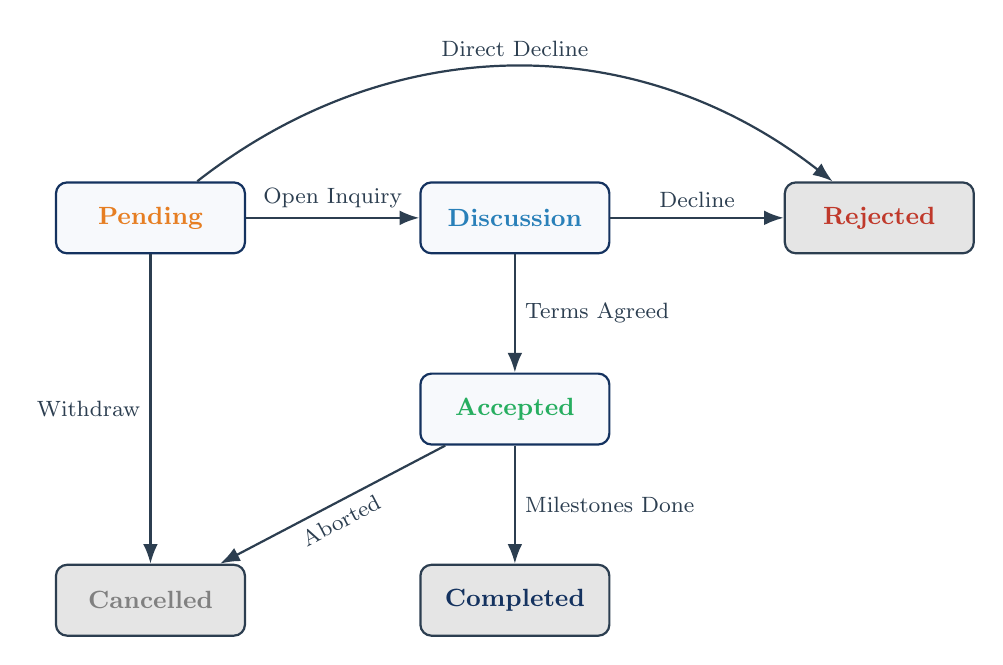
\begin{tikzpicture}[
    node distance=1.5cm and 2.2cm,
    state/.style={rectangle, rounded corners, draw=primary, fill=lightbg, thick, minimum width=2.4cm, minimum height=0.9cm, align=center, font=\small\bfseries},
    terminal/.style={rectangle, rounded corners, draw=darkslate, fill=gray!20, thick, minimum width=2.4cm, minimum height=0.9cm, align=center, font=\small\bfseries},
    arrow/.style={-{Latex[length=2.5mm]}, thick, color=darkslate}
]
    \node[state] (pending) {\textcolor{accent}{Pending}};
    \node[state, right=of pending] (discussion) {\textcolor{secondary}{Discussion}};
    \node[state, below=of discussion] (accepted) {\textcolor{badgegreen}{Accepted}};
    \node[terminal, right=of discussion] (rejected) {\textcolor{badgered}{Rejected}};
    \node[terminal, below=of accepted] (completed) {\textcolor{primary}{Completed}};
    \node[terminal, left=of completed] (cancelled) {\textcolor{gray}{Cancelled}};

    \draw[arrow] (pending) -- node[above, font=\footnotesize] {Open Inquiry} (discussion);
    \draw[arrow] (pending) -- node[left, font=\footnotesize] {Withdraw} (cancelled);
    \draw[arrow] (pending) to[bend left=38] node[above, font=\footnotesize] {Direct Decline} (rejected);
    \draw[arrow] (discussion) -- node[right, font=\footnotesize] {Terms Agreed} (accepted);
    \draw[arrow] (discussion) -- node[above, font=\footnotesize] {Decline} (rejected);
    \draw[arrow] (accepted) -- node[right, font=\footnotesize] {Milestones Done} (completed);
    \draw[arrow] (accepted) -- node[below, sloped, font=\footnotesize] {Aborted} (cancelled);
\end{tikzpicture}
\caption{Finite State Machine for Collaboration Request Lifecycle}
\label{fig:fsm_collab}
\end{figure}

\subsubsection{Feature 9: Research Team Builder}
Allows students to configure required multidisciplinary roles for complex capstone projects. The AI engine evaluates prospective candidates simultaneously, optimizing for collective skill coverage, schedule compatibility, and complementary expertise while proactively alerting students to vacant competencies.

\subsubsection{Feature 10: AI Research Requirement Assistant}
An interactive conversational assistant designed to help novice students refine ambiguous research inquiries prior to expert outreach. The assistant identifies missing methodologies, breaks the project into structured milestones, and drafts professional, highly compelling collaboration proposals.

\subsubsection{Feature 11: Side-by-Side Expert Comparison Engine}
Provides students with an objective comparative dashboard evaluating candidate experts across orthogonal dimensions: skill overlap percentage, publication count in the specific subfield, verified status, availability score, and past student rating distributions.

\subsubsection{Feature 12: Integrated Workspace and Discussion Channels}
Upon request acceptance, the platform automatically provisions a secure collaboration workspace featuring thread-based asynchronous messaging, document and proposal attachment sharing, milestone tracking, and calendar meeting coordination.

% ------------------------------------------------------------------------------
% SECTION 4: ADVANCED AI/ML ARCHITECTURE & FORMULATION
% ------------------------------------------------------------------------------
\section[Advanced AI/ML Architecture]{Advanced AI/ML Recommendation Architecture}
\label{sec:aiml_engine}

To fulfill the rigorous software engineering and computer science research requirements of a capstone, UniExpert introduces a multi-stage hybrid retrieval and ranking pipeline.

\subsection{The Hybrid Matching Model Formulation}
Given a student research problem profile $u$ and a candidate expert profile $e \in \mathcal{E}$, the ranking engine computes a composite compatibility score $\mathcal{S}(u, e) \in [0, 1]$ via a multi-criteria linear weighting scheme:

\begin{equation}
    \mathcal{S}(u, e) = w_1 \cdot \mathcal{D}(u, e) + w_2 \cdot \mathcal{S}_{\text{skill}}(u, e) + w_3 \cdot \mathcal{R}_{\text{sim}}(u, e) + w_4 \cdot \mathcal{E}_{\text{evid}}(e) + w_5 \cdot \mathcal{A}(u, e) + w_6 \cdot \mathcal{C}(u, e)
    \label{eq:hybrid_formula}
\end{equation}

Subject to the convex optimization constraint:
\begin{equation}
    \sum_{i=1}^{6} w_i = 1.0 \quad \text{where} \quad w_i \ge 0 \quad \forall i \in \{1, \dots, 6\}
\end{equation}

The individual constituent normalized metrics are defined as follows:

\begin{enumerate}[label=\textbf{\arabic*.}]
    \item \textbf{Domain Relevance $\mathcal{D}(u, e) \in [0, 1]$:} Measures taxonomic alignment across the hierarchical academic tree $\mathcal{T}$:
    \begin{equation}
        \mathcal{D}(u, e) = \frac{2 \cdot \text{depth}(\text{LCA}(d_u, d_e))}{\text{depth}(d_u) + \text{depth}(d_e)}
    \end{equation}
    where $\text{LCA}(d_u, d_e)$ denotes the Lowest Common Ancestor of the project's required domain $d_u$ and the expert's primary domain $d_e$ within the knowledge taxonomy.

    \item \textbf{Skill Compatibility $\mathcal{S}_{\text{skill}}(u, e) \in [0, 1]$:} Evaluates the intersection of required project skills $\mathcal{K}_u$ and the expert's validated skills $\mathcal{K}_e$ using a weighted soft Jaccard index:
    \begin{equation}
        \mathcal{S}_{\text{skill}}(u, e) = \frac{\sum_{k \in \mathcal{K}_u \cap \mathcal{K}_e} \omega_k}{\sum_{k \in \mathcal{K}_u \cup \mathcal{K}_e} \omega_k}
    \end{equation}
    where $\omega_k$ represents the inverse document frequency (IDF) weight of skill $k$ across the global expert corpus.

    \item \textbf{Semantic Research Interest Similarity $\mathcal{R}_{\text{sim}}(u, e) \in [0, 1]$:} Dense vector cosine similarity between the dense embedding of the student's problem text $\mathbf{v}_u$ and the candidate expert's aggregated research dossier $\mathbf{v}_e$ (composed of bio, publications, and thesis abstracts):
    \begin{equation}
        \mathcal{R}_{\text{sim}}(u, e) = \max\left(0, \frac{\mathbf{v}_u \cdot \mathbf{v}_e}{\|\mathbf{v}_u\|_2 \|\mathbf{v}_e\|_2}\right)
    \end{equation}
    where $\mathbf{v} \in \mathbb{R}^{d}$ is computed via a fine-tuned dense sentence transformer (e.g., Sentence-BERT \cite{reimers2019sentence} or \texttt{SciBERT} \cite{beltagy2019scibert}).

    \item \textbf{Evidence and Verified Experience $\mathcal{E}_{\text{evid}}(e) \in [0, 1]$:} Quantifies verified credibility rather than self-reported claims:
    \begin{equation}
        \mathcal{E}_{\text{evid}}(e) = \alpha \cdot V_{\text{badge}}(e) + (1 - \alpha) \cdot \min\left(1.0, \frac{\log(1 + N_{\text{pub}}(e))}{\log(1 + N_{\text{max}})}\right)
    \end{equation}
    where $V_{\text{badge}}(e) \in \{0.25, 0.5, 0.75, 1.0\}$ corresponds to the verified tier level, and $N_{\text{pub}}(e)$ is the count of verified peer-reviewed publications.

    \item \textbf{Availability Compatibility $\mathcal{A}(u, e) \in [0, 1]$:} Evaluates the overlap between the student's expected project schedule $T_u$ (hours/week and duration) and the expert's active availability capacity $T_e$:
    \begin{equation}
        \mathcal{A}(u, e) = 1.0 - \frac{|T_u - T_e|}{\max(T_u, T_e, 1)}
    \end{equation}

    \item \textbf{Collaboration Preference Compatibility $\mathcal{C}(u, e) \in [0, 1]$:} Binary indicator or multi-class match evaluating requested collaboration modality (e.g., Virtual, In-Person, Advisory, Co-Author).
\end{enumerate}

\subsection{Explainable Recommendations (Feature 14)}
Trust in AI-driven matching requires complete transparency. For each recommended candidate, UniExpert's Explainable AI (XAI) engine constructs a structured natural language breakdown:
\begin{itemize}
    \item \textbf{Positive Feature Attribution:} Highlighting specific matching skills (e.g., \textit{``Matches 4/4 required skills: PyTorch, YOLOv8, Image Segmentation, Transfer Learning''}).
    \item \textbf{Corroborating Evidence:} Citing specific verified publications (e.g., \textit{``Authored: `Automated Lesion Detection in Avian Flocks (2024)' in Journal of Poultry Science''}).
    \item \textbf{Identified Gaps:} Explicitly identifying missing or unverified competencies (e.g., \textit{``Note: Candidate has no recorded publications in Veterinary Pharmacology; experience in field data collection is self-reported''}).
\end{itemize}

\subsection{Skill Gap Detection Engine (Feature 15)}
When constructing multi-member research teams, the platform evaluates collective skill sets using a set-cover algorithm. Given project requirements $\mathcal{K}_u$ and the set of accepted team members $\mathcal{M} = \{e_1, e_2, \dots, e_m\}$, the missing skill set $\Delta \mathcal{K}$ is computed as:
\begin{equation}
    \label{eq:team_skill_gap}
    \Delta \mathcal{K} = \mathcal{K}_u \setminus \bigcup_{e \in \mathcal{M}} \mathcal{K}_e
\end{equation}
If $|\Delta \mathcal{K}| > 0$, the platform immediately invokes targeted sub-searches specifically calibrated to minimize $|\Delta \mathcal{K}|$ with the minimum number of additional recruits.

% ------------------------------------------------------------------------------
% SECTION 5: SYSTEM ARCHITECTURE & TECHNICAL STACK
% ------------------------------------------------------------------------------
\section{System Architecture and Implementation Stack}

\subsection{High-Level Architectural Blueprint}
UniExpert adopts a modular, service-oriented architecture ensuring separation of concerns, rapid testing, and independent scaling of heavy ML inference workloads. Figure~\ref{fig:architecture} presents the comprehensive system topology.

\begin{figure}[htbp]
\centering
\resizebox{0.95\linewidth}{!}{%
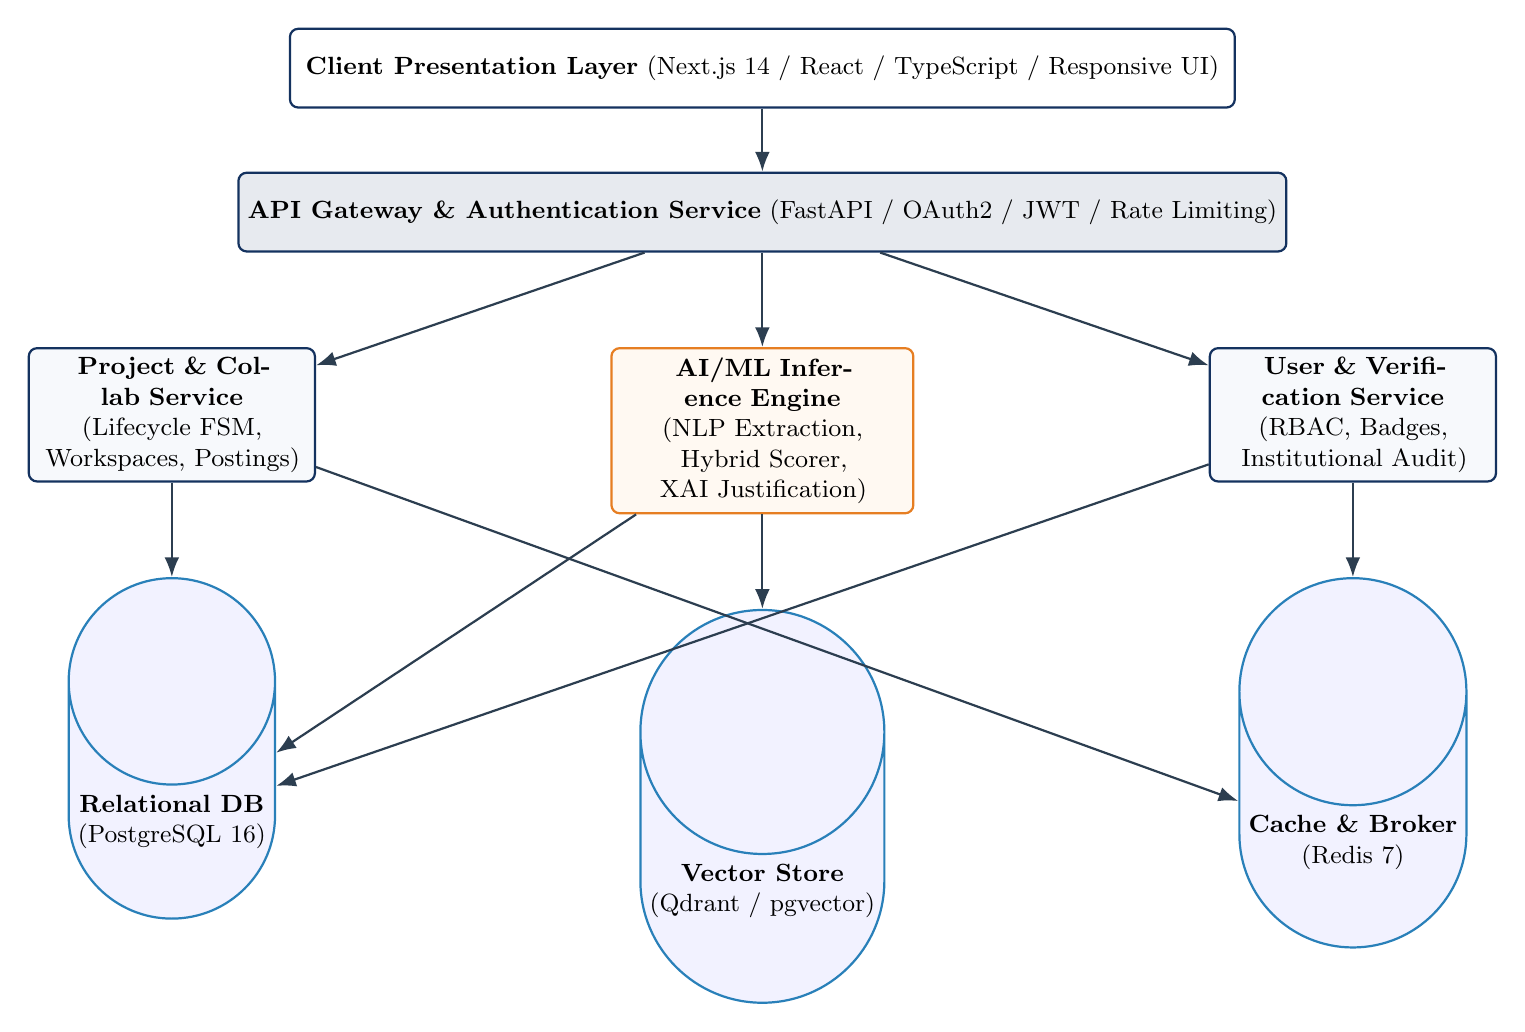
\begin{tikzpicture}[
    box/.style={rectangle, draw=primary, fill=lightbg, rounded corners=3pt, thick, align=center, font=\small, minimum height=1cm},
    databox/.style={cylinder, shape border rotate=90, draw=secondary, fill=blue!5, thick, align=center, font=\small, minimum height=1.1cm, minimum width=2.0cm},
    aibox/.style={rectangle, draw=accent, fill=orange!5, rounded corners=3pt, thick, align=center, font=\small, minimum height=1cm},
    arrow/.style={-{Latex[length=2.5mm]}, thick, color=darkslate}
]
    % Client Layer
    \node[box, fill=white, minimum width=12cm] (client) {\textbf{Client Presentation Layer} (Next.js 14 / React / TypeScript / Responsive UI)};

    % Gateway
    \node[box, below=0.8cm of client, minimum width=12cm, fill=primary!10] (gateway) {\textbf{API Gateway \& Authentication Service} (FastAPI / OAuth2 / JWT / Rate Limiting)};

    % Application Services
    \node[box, below left=1.2cm and -1.0cm of gateway, text width=3.4cm] (projectsvc) {\textbf{Project \& Collab Service}\\(Lifecycle FSM, Workspaces, Postings)};
    \node[aibox, below=1.2cm of gateway, text width=3.6cm] (aisvc) {\textbf{AI/ML Inference Engine}\\(NLP Extraction, Hybrid Scorer, XAI Justification)};
    \node[box, below right=1.2cm and -1.0cm of gateway, text width=3.4cm] (authsvc) {\textbf{User \& Verification Service}\\(RBAC, Badges, Institutional Audit)};

    % Data Layer
    \node[databox, below=1.2cm of projectsvc] (postgres) {\textbf{Relational DB}\\(PostgreSQL 16)};
    \node[databox, below=1.2cm of aisvc] (vectordb) {\textbf{Vector Store}\\(Qdrant / pgvector)};
    \node[databox, below=1.2cm of authsvc] (redis) {\textbf{Cache \& Broker}\\(Redis 7)};

    % Connections
    \draw[arrow] (client) -- (gateway);
    \draw[arrow] (gateway) -- (projectsvc);
    \draw[arrow] (gateway) -- (aisvc);
    \draw[arrow] (gateway) -- (authsvc);

    \draw[arrow] (projectsvc) -- (postgres);
    \draw[arrow] (projectsvc) -- (redis);
    \draw[arrow] (aisvc) -- (vectordb);
    \draw[arrow] (aisvc) -- (postgres);
    \draw[arrow] (authsvc) -- (postgres);
    \draw[arrow] (authsvc) -- (redis);
\end{tikzpicture}%
}
\caption{UniExpert High-Level System Architecture}
\label{fig:architecture}
\end{figure}

\subsection{Technology Stack Selection and Justification}
Table~\ref{tab:tech_stack} outlines the technological framework selected for the implementation of the UniExpert platform.

\begin{table}[htbp]
\centering
\small
\caption{Technology Stack Specifications and Architectural Rationale}
\label{tab:tech_stack}
\begin{tabularx}{\textwidth}{@{}l p{3.2cm} X@{}}
\toprule
\textbf{Layer} & \textbf{Selected Technology} & \textbf{Engineering Justification} \\
\midrule
\textbf{Frontend Client} & Next.js 14 / React / TypeScript / Modern CSS & Server-Side Rendering (SSR) for fast loading, strong static typing, reactive component architecture, and modern responsive layouts. \\
\addlinespace
\textbf{Backend REST API} & FastAPI (Python 3.11) & Native asynchronous execution, automated OpenAPI documentation, high throughput, and seamless integration with Python ML pipelines. \\
\addlinespace
\textbf{AI \& NLP Core} & HuggingFace Transformers, PyTorch, SciBERT & State-of-the-art transformer architectures for domain classification, dense sentence embeddings, and token-level skill extraction. \\
\addlinespace
\textbf{Dense Vector Store} & Qdrant / \texttt{pgvector} & Ultra-low latency Approximate Nearest Neighbor (ANN) vector indexing via HNSW graphs; scales to hundreds of thousands of expert vectors. \\
\addlinespace
\textbf{Primary Database} & PostgreSQL 16 & ACID compliance, rich JSONB support for dynamic profile portfolios, and robust relational integrity for user authentication and request FSMs. \\
\addlinespace
\textbf{Caching \& Queues} & Redis 7 & Session state caching, rate limiting, and asynchronous message broker for background embedding indexing jobs. \\
\bottomrule
\end{tabularx}
\end{table}

% ------------------------------------------------------------------------------
% SECTION 6: RESEARCH METHODOLOGY AND ML EVALUATION
% ------------------------------------------------------------------------------
\section[Research Methodology \& Evaluation]{Research Methodology and AI/ML Evaluation Plan}

A critical requirement of an academic Software Engineering capstone is rigorous empirical evaluation. UniExpert is designed not merely as a commercial web utility, but as a research-grade artifact testing formal scientific hypotheses.

\subsection{Primary Research Questions}
\begin{itemize}
    \item \textbf{RQ1:} \textit{Does a multi-criteria hybrid recommendation model yield statistically significant higher recommendation accuracy (Precision@5 and NDCG@5) compared to baseline keyword retrieval (BM25) and dense semantic vector similarity alone?}
    \item \textbf{RQ2:} \textit{To what degree does automated natural language skill extraction align with expert human-annotated requirements across interdisciplinary capstone problem statements?}
    \item \textbf{RQ3:} \textit{Do explainable recommendation justifications increase student trust and collaboration request conversion rates compared to unadorned similarity scores?}
\end{itemize}

\subsection{Experimental Baseline Comparisons}
To evaluate the recommendation engine objectively, we implement and benchmark three competing retrieval pipelines under identical corpus conditions:
\begin{enumerate}
    \item \textbf{Baseline A (Lexical Matching):} Classical BM25 keyword search over tokenized expert profile resumes and publication titles.
    \item \textbf{Baseline B (Dense Semantic Retrieval):} Pure bi-encoder sentence embedding cosine similarity ($\mathcal{R}_{\text{sim}}$) without skill weighting or evidence filtering.
    \item \textbf{Proposed Method (UniExpert Hybrid):} Multi-criteria weighted ranking engine incorporating domain taxonomy, skill IDF Jaccard, semantic similarity, verified evidence tiers, and schedule compatibility (Eq.~\ref{eq:hybrid_formula}).
\end{enumerate}

\subsection{Evaluation Metrics}
The quantitative performance of the retrieval pipelines will be benchmarked using the standard Information Retrieval (IR) metrics defined below:

\begin{table}[htbp]
\centering
\small
\caption{Formal Evaluation Metrics for Recommendation Performance}
\label{tab:metrics}
\begin{tabularx}{\textwidth}{@{}l p{4.2cm} X@{}}
\toprule
\textbf{Metric} & \textbf{Mathematical Definition} & \textbf{Evaluation Objective} \\
\midrule
\textbf{Precision@$K$} & $\text{P}@K = \frac{|\text{Relevant Experts in Top-}K|}{K}$ & Measures the proportion of relevant experts appearing in the top-$K$ recommendations ($K \in \{5, 10\}$). \\
\addlinespace
\textbf{Recall@$K$} & $\text{R}@K = \frac{|\text{Relevant Experts in Top-}K|}{|\text{All Known Relevant Experts}|}$ & Measures the engine's ability to retrieve all suitable candidates from the dataset. \\
\addlinespace
\textbf{NDCG@$K$} & $\text{NDCG}@K = \frac{\text{DCG}@K}{\text{IDCG}@K}$ where $\text{DCG}@K = \sum_{i=1}^K \frac{2^{rel_i}-1}{\log_2(i+1)}$ & Evaluates ranking quality, heavily penalizing relevant experts placed low in the result list. \\
\addlinespace
\textbf{Skill Extraction F1} & $\text{F1} = 2 \cdot \frac{\text{Precision} \cdot \text{Recall}}{\text{Precision} + \text{Recall}}$ & Evaluates the NLP token extraction accuracy against human gold-standard annotations. \\
\addlinespace
\textbf{System Latency} & $p_{50}, p_{95}, p_{99}$ response times (ms) & Validates real-time responsiveness and engineering throughput of the vector index. \\
\bottomrule
\end{tabularx}
\end{table}

\subsection{Dataset Construction and Human Relevance Judgment}
To avoid synthetic bias, an evaluation dataset comprising 100 authentic, anonymized capstone problem descriptions spanning five faculties (Engineering, Agriculture, Business, Health Sciences, and Humanities) will be constructed. A pool of 300 consenting expert profiles (professors, researchers, alumni) will be seeded. 
A panel of qualified academic evaluators (senior faculty members and researchers) will perform blind graded relevance assessments on a 3-point Likert scale (0: Irrelevant, 1: Partially Relevant, 2: Highly Relevant). Inter-rater agreement will be validated using Cohen's Kappa ($\kappa \ge 0.70$).

% ------------------------------------------------------------------------------
% SECTION 7: TRUST, SAFETY, AND ALGORITHMIC FAIRNESS
% ------------------------------------------------------------------------------
\section[Trust, Safety \& Fairness]{Trust, Safety, Privacy, and Algorithmic Fairness}

\subsection{Anti-Bias and Fair Matching Principles (Feature 25)}
A recognized hazard in academic recommender systems is the \textit{Matthew Effect} (``rich get richer''), wherein senior, highly cited scholars receive all recommendation traffic while junior faculty and early-career researchers remain undiscovered. UniExpert incorporates explicit algorithmic fairness safeguards:
\begin{itemize}
    \item \textbf{Popularity De-biasing:} The scoring function avoids raw profile view counts or global popularity as an input metric.
    \item \textbf{Cold-Start Exploration Boost:} A randomized contextual $\epsilon$-greedy exploration mechanism allocates 10\% of top recommendation slots to newly registered, fully verified experts possessing high skill overlap.
    \item \textbf{Protected Attributes Blindness:} Sensitive personal attributes (gender, age, ethnicity, national origin) are strictly excluded from all vector indexing and ranking formulas.
\end{itemize}

\subsection{Privacy Controls and Data Governance (Feature 23)}
All platform interactions adhere strictly to academic data protection standards. Students can designate project descriptions as Private or Protected. Direct contact details (telephone numbers, personal emails) are masked behind the platform's workspace abstraction until explicit collaboration acceptance is confirmed by both parties.

\clearpage
% ------------------------------------------------------------------------------
% SECTION 8: IMPLEMENTATION SCOPE & MOSCOW PRIORITIZATION
% ------------------------------------------------------------------------------
\section[Implementation Scope \& MoSCoW]{Implementation Scope and MVP Prioritization}

To guarantee successful project delivery within the Fall 2026 semester timeframe (October -- December 2026, 12 weeks), features are strictly triaged using the MoSCoW prioritization model, as detailed in Table~\ref{tab:moscow}.

\begin{table}[H]
\centering
\small
\caption{MoSCoW Feature Scope Prioritization for Fall 2026 (October -- December 2026)}
\label{tab:moscow}
\begin{tabularx}{\textwidth}{@{}p{2.8cm} X p{3.2cm}@{}}
\toprule
\textbf{Classification} & \textbf{Feature Scope \& Description} & \textbf{Delivery Target} \\
\midrule
\textbf{Must-Have} \newline (Core MVP) & 
\begin{itemize}[leftmargin=*,noitemsep]
    \item Student and expert registration with role-based auth.
    \item Rich student and expert profiles with skill taxonomy.
    \item Multi-tier expert verification workflow (email \& documents).
    \item Natural language project submission \& NLP skill extractor.
    \item Semantic dense vector search and hybrid multi-criteria ranker.
    \item Explainable natural language recommendation justifications.
    \item Collaboration request management (FSM) \& basic messaging.
    \item Administrative supervision dashboard \& empirical evaluation.
\end{itemize} & \textbf{October -- November 2026} \newline (Weeks 1--8) \\
\addlinespace
\textbf{Should-Have} \newline (Extended Scope) & 
\begin{itemize}[leftmargin=*,noitemsep]
    \item Multidisciplinary problem decomposition \& team builder.
    \item Automated skill gap detection for project teams.
    \item Side-by-side expert comparison matrix.
    \item Automated Google Scholar / ORCID public metadata sync.
    \item Structured post-collaboration ratings and feedback.
\end{itemize} & \textbf{December 2026} \newline (Weeks 9--12) \\
\addlinespace
\textbf{Could-Have} \newline (Future Work) & 
\begin{itemize}[leftmargin=*,noitemsep]
    \item Integrated real-time WebRTC video conference rooms.
    \item Institutional cross-campus analytics federation.
    \item Paid consultation escrow and honorarium management.
    \item Native mobile applications (iOS/Android).
\end{itemize} & Post-Capstone / Future Research \\
\bottomrule
\end{tabularx}
\end{table}

\clearpage
% ------------------------------------------------------------------------------
% SECTION 9: SEMESTER DEVELOPMENT PLAN AND GANTT SCHEDULE
% ------------------------------------------------------------------------------
\section[Semester Plan \& Timeline]{Semester Development Plan and Milestones (Fall 2026)}

The capstone project spans a disciplined 12-week Fall 2026 semester execution schedule (October -- December 2026), structured across three distinct monthly milestones, as synthesized in Table~\ref{tab:gantt_table}.

\begin{table}[H]
\centering
\small
\caption{Fall 2026 (October -- December 2026) Capstone Development Timeline and Deliverables}
\label{tab:gantt_table}
\begin{tabularx}{\textwidth}{@{}p{2.5cm} p{1.8cm} X p{3.4cm}@{}}
\toprule
\textbf{Phase} & \textbf{Duration} & \textbf{Key Engineering Deliverables \& Research Activities} & \textbf{Milestone} \\
\midrule
\textbf{Month 1} \newline (October 2026) & Weeks 1--4 & 
\begin{itemize}[leftmargin=*,noitemsep]
    \item Formalize Software Requirements Specification (SRS) and architecture.
    \item Literature review of expert finding and recommender systems.
    \item Stakeholder interviews with faculty advisors and student researchers.
    \item PostgreSQL relational schema, Redis cache design, and API contracts.
    \item Git repository governance, automated linting, and CI/CD pipelines.
\end{itemize} & \textbf{M1: System Blueprint} \newline (Requirements \& Architecture) \\
\addlinespace
\textbf{Month 2} \newline (November 2026) & Weeks 5--8 & 
\begin{itemize}[leftmargin=*,noitemsep]
    \item Implement OAuth2/JWT authentication and RBAC security services.
    \item Student and expert profile schemas, portfolio UI, and verification.
    \item Natural language project parsing and NLP skill extraction pipeline.
    \item Qdrant vector database integration with dense sentence embeddings.
    \item Hybrid multi-criteria ranking model (Eq.~\ref{eq:hybrid_formula}) and XAI explanations.
    \item Collaboration request state machine (FSM) and workspace channels.
\end{itemize} & \textbf{M2: Core Platform \& AI Matchmaking Engine} \\
\addlinespace
\textbf{Month 3} \newline (December 2026) & Weeks 9--12 & 
\begin{itemize}[leftmargin=*,noitemsep]
    \item Multidisciplinary team builder and skill gap optimizer (Eq.~\ref{eq:team_skill_gap}).
    \item Empirical IR comparative evaluation (BM25 vs. Vector vs. Hybrid).
    \item System integration, end-to-end security audits, and UAT with users.
    \item Comprehensive capstone thesis report, documentation, and final defense.
\end{itemize} & \textbf{M3: Empirical Evaluation \& Final Defense} \\
\bottomrule
\end{tabularx}
\end{table}

\clearpage
% ------------------------------------------------------------------------------
% SECTION 10: RISK ASSESSMENT AND MITIGATION STRATEGIES
% ------------------------------------------------------------------------------
\section[Risk Assessment \& Mitigation]{Risk Assessment and Mitigation Strategies}

A rigorous engineering proposal must preemptively identify technical and organizational hazards. Table~\ref{tab:risks} formalizes the risk matrix and corresponding mitigation protocols.

\begin{table}[H]
\centering
\small
\caption{Comprehensive Project Risk Matrix and Mitigation Strategies}
\label{tab:risks}
\begin{tabularx}{\textwidth}{@{}p{3.0cm} c c X@{}}
\toprule
\textbf{Identified Risk} & \textbf{Likelihood} & \textbf{Impact} & \textbf{Engineered Mitigation Protocol} \\
\midrule
\textbf{Data Cold-Start} \newline (Scarce initial profiles) & High & High & Pre-seed database with public faculty profiles from consenting departments; implement automated ORCID/Google Scholar import utilities. \\
\addlinespace
\textbf{NLP Extraction Hallucination} & Med & Med & Combine regex-based taxonomy dictionary matching with zero-shot transformer classifiers; provide interactive UI allowing students to verify extracted skills. \\
\addlinespace
\textbf{Vector Search Latency} & Low & High & Pre-compute embeddings asynchronously; utilize HNSW indexing in Qdrant; cache top domain search clusters in Redis. \\
\addlinespace
\textbf{Credential Falsification} & Med & High & Enforce institutional email verification (\texttt{.edu}); display distinct, unforgeable badge indicators separating verified records from claims. \\
\addlinespace
\textbf{Faculty Availability Fatigue} & High & Med & Implement monthly request quotas per expert; provide automated calendar blackout toggles; enable one-click polite declination templates. \\
\bottomrule
\end{tabularx}
\end{table}

% ------------------------------------------------------------------------------
% SECTION 11: CONCLUSION AND EXPECTED CAPSTONE OUTCOMES
% ------------------------------------------------------------------------------
\section[Conclusion \& Deliverables]{Conclusion and Expected Capstone Outcomes}

The \textbf{UniExpert} platform addresses an urgent, unfulfilled need in higher education: breaking down academic silos to connect university researchers and students through transparent, AI-driven expert discovery. By departing from rigid keyword indexes and pioneering a problem-driven, multi-criteria recommendation architecture, UniExpert empowers students to find the exact mentorship necessary to elevate their capstone projects from standard coursework into high-impact academic contributions.

Upon successful completion of this Fall 2026 capstone project (October -- December 2026), the expected academic and engineering deliverables comprise:
\begin{enumerate}
    \item A fully functional, production-ready, accessible web platform conforming to modern software engineering standards.
    \item An empirical research dataset and benchmarking suite establishing quantitative improvements in recommendation quality over classical IR baselines.
    \item A comprehensive capstone thesis report and a submission-ready research paper targeted at academic software engineering and educational technology venues.
    \item A scalable foundation for institutional adoption across university departments.
\end{enumerate}

% ------------------------------------------------------------------------------
% REFERENCES / BIBLIOGRAPHY
% ------------------------------------------------------------------------------
\begin{thebibliography}{99}
\addcontentsline{toc}{section}{References}

\bibitem{balog2012expertise}
K.~Balog,
\emph{Expertise Retrieval: A Survey},
Foundations and Trends in Information Retrieval, vol.~6, no.~2--3, pp.~127--256, 2012.

\bibitem{reimers2019sentence}
N.~Reimers and I.~Gurevych,
\emph{Sentence-BERT: Sentence Embeddings using Siamese BERT-Networks},
in Proceedings of the 2019 Conference on Empirical Methods in Natural Language Processing (EMNLP), pp.~3982--3992, 2019.

\bibitem{karpukhin2020dense}
V.~Karpukhin, B.~O{\u{g}}uz, S.~Min, P.~Lewis, L.~Wu, S.~Edunov, D.~Chen, and W.-t.~Yih,
\emph{Dense Passage Retrieval for Open-Domain Question Answering},
in Proceedings of the 2020 Conference on Empirical Methods in Natural Language Processing (EMNLP), pp.~6769--6781, 2020.

\bibitem{lappas2009finding}
T.~Lappas, K.~Liu, and E.~Terzi,
\emph{Finding a Team of Experts in Social Networks},
in Proceedings of the 15th ACM SIGKDD International Conference on Knowledge Discovery and Data Mining (KDD), pp.~467--476, 2009.

\bibitem{tintarev2015explaining}
N.~Tintarev and J.~Masthoff,
\emph{Explaining Recommendations: Design and Evaluation},
in Recommender Systems Handbook, F.~Ricci, L.~Rokach, and B.~Shapira, Eds., Springer, pp.~353--382, 2015.

\bibitem{robertson2009probabilistic}
S.~Robertson and H.~Zaragoza,
\emph{The Probabilistic Relevance Framework: BM25 and Beyond},
Foundations and Trends in Information Retrieval, vol.~3, no.~4, pp.~333--389, 2009.

\bibitem{beltagy2019scibert}
I.~Beltagy, K.~Lo, and A.~Cohan,
\emph{SciBERT: A Pretrained Language Model for Scientific Text},
in Proceedings of the 2019 Conference on Empirical Methods in Natural Language Processing (EMNLP), pp.~3615--3620, 2019.

\end{thebibliography}

\end{document}
